%!TEX root = main.tex

\chapter{Results and Analysis}

	This chapter discusses the quantitative and qualitative results of the testing from the several iterations. The analysis of the results and improvements made in accordance to those results are also discussed in this chapter.

	\section{Preliminary Results}
		During the first two (2) iterations, five (5) subjects of both genders aged 18-40 were recruited through snowball sampling method to take part in the data collection and testing. These subjects were categorized into two (2) user groups based on musical composition experience: amateur, and experienced.

		Table \ref{tab:results-features-it1} lists an overview of the results from the questionnaire given after performing the test setups in Iteration 1 while tables \ref{tab:results-features-it2} and \ref{tab:clerical-features} list the results from Iteration 2. As mentioned before, answers are on a scale of 1 - 4, 1 (Never or Strongly Disagree) being the lowest, and 4 (Frequently or Strongly Agree) being the highest for Iteration 1. Since there were more features in Iteration 2, there was an added option of 0 (N/A) for features that were not used during the testing. Each of the questions are repeated for each feature.

		\subsection{Iteration 1} 

			\begin{table}[!htpb]
			  \centering
			  \captionof{table}{Feature Related Questions for Iteration 1} \label{tab:results-features-it1}
			  \begin{tabular}{|R{1.5cm}|R{1cm}|R{1cm}|R{1cm}|R{1cm}|R{1cm}|R{1.5cm}|}
			  	\hline
			  	& \textbf{Q1} & \textbf{Q2} & \textbf{Q3} & \textbf{Q4} & \textbf{Q5} & \textbf{AveF} \\ 
			    \hline
			    \textbf{F1} & 4.0 		& 3.2 	& 2.6 	& 3.4 	& 2.0 	& 3.04 \\ \hline
			    \textbf{F2} & 2.2 		& 1.8 	& 2.0 	& 3.0 	& 1.8 	& \textbf{2.16} \\ \hline
			    \textbf{F3} & 2.0 		& 1.8 	& 1.8 	& 3.2 	& 2.4 	& 2.24 \\ \hline
			    \textbf{F4} & 4.0 		& 4.0 	& 3.4 	& 3.6 	& 3.4 	& \textbf{3.68} \\ \hline
			    \textbf{F5} & 3.8 		& 3.2 	& 3.6 	& 3.4 	& 3.0 	& 3.40 \\ \hline
			   	\textbf{F6} & 2.4 		& 2.0 	& 1.8 	& 3.2 	& 2.8 	& 2.44 \\ \hline
			    \textbf{F7} & 2.4 		& 1.8 	& 2.2 	& 2.4 	& 2.4 	& 2.24 \\ \hline
			    \textbf{F8} & 2.2 		& 1.8 	& 2.2 	& 2.4 	& 2.2 	& \textbf{2.16} \\
			    
			    \hline
			    \textbf{AveQ} & 2.88 & 2.45 & 2.45 & 3.08 & 2.50 & \\
			    \hline
			  \end{tabular}
			\end{table}

			From the data gathered and analyzed, a clear difference in respondent sentiment was observed from features that needed multiple note selection (see F2 and F8) versus those that did not. This is most notable in the edit and delete features which had the lowest scores on average. Both of these features required the selection feature. Most of the respondents were not able to figure out and correctly execute the gesture for selection which was a two-finger drag. Although it is common for mobile applications to use one-finger drag to scroll, the results suggest otherwise. It was found that the gesture for highlighting (two-finger drag) would have felt more natural if it was switched with the scroll gesture (one-finger drag). Hence, for the second iteration, the gestures for these interactions were switched (see Figure \ref{fig:highlight}).

			\begin{figure}[h]
				\centering
				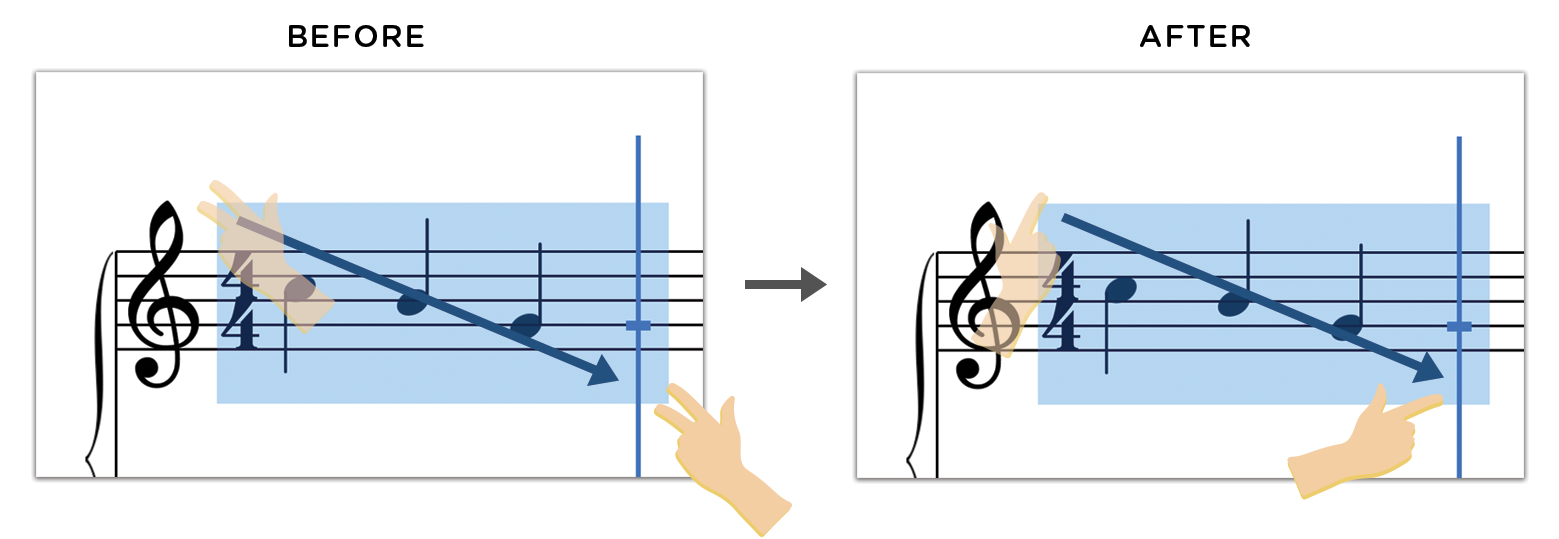
\includegraphics[scale=0.25]{figures/before-after-highlight}
			    \caption{The highlight interaction before and after changes were made due to the user testing. The new interaction uses only one (1) finger.}
			    \label{fig:highlight}
			\end{figure}

			Other than the note selection feature, respondents have expressed that most of the features worked well and felt comfortable to use. Although it was not like how they would regularly write music (i.e. pen and paper), Flow's method of composing was easy to learn and get used to. Majority liked the ease of using the cursor/indicator because they can simply tap on the location they want or use the arrow keys when they want to be accurate.

		\subsection{Iteration 2}

			\begin{table}[!htpb]
			  \centering
			  \captionof{table}{Feature Related Questions for Iteration 2} \label{tab:results-features-it2}
			  \begin{tabular}{|R{1.5cm}|R{1cm}|R{1cm}|R{1cm}|R{1cm}|R{1cm}|R{1.5cm}|}
			  	\hline
			  	& \textbf{Q1} & \textbf{Q2} & \textbf{Q3} & \textbf{Q4} & \textbf{Q5} & \textbf{AveF} \\ \hline
			    \textbf{F1} & 3.8 		& 3.6 	& 3.2 	& 3.8 	& 3.4 	& \cellcolor{green!25} 3.56 \\ \hline
			    \textbf{F2} & 3.4 		& 3.2 	& 3.0 	& 3.2 	& 3.2 	& \cellcolor{green!25} 3.20 \\ \hline
			    \textbf{F3} & 3.8 		& 3.8 	& 3.2 	& 3.8 	& 3.8 	& \cellcolor{green!25} 3.68 \\ \hline
			    \textbf{F4} & 4.0 		& 3.6 	& 3.2 	& 3.6 	& 3.8 	& \cellcolor{red!25} 3.64 \\ \hline
			    \textbf{F5} & 4.0 		& 3.4 	& 3.0 	& 3.6 	& 3.4 	& \cellcolor{green!25} 3.48 \\ \hline
			    \textbf{F6} & 4.0 		& 4.0 	& 3.4 	& 3.8 	& 4.0 	& \cellcolor{green!25} 3.84 \\ \hline
			    \textbf{F7} & 2.2 		& 3.6 	& 3.4 	& 3.6 	& 3.6 	& \cellcolor{green!25} 3.28 \\ \hline
			    \textbf{F8} & 3.2 		& 4.0 	& 4.0 	& 4.0 	& 4.0 	& \cellcolor{green!25} 3.84 \\ \hline
			    \textbf{F9} & 3.8 		& 3.6 	& 2.8 	& 3.8 	& 3.6 	& 3.52 \\ \hline
			    \textbf{F10} & 3.2 		& 3.4 	& 2.4 	& 3.8 	& 3.0 	& 3.16 \\ \hline
			    \textbf{F11} & 3.4 		& 3.6 	& 3.2 	& 3.6 	& 3.6 	& 3.48 \\ \hline
			    \textbf{F12} & 3.8 		& 3.8 	& 3.8 	& 3.8 	& 3.8 	& 3.80 \\ \hline
			    \textbf{F13} & 3.2 		& 2.4 	& 2.6 	& 2.4 	& 3.0 	& 2.72 \\ \hline
			    \textbf{F14} & 2.2 		& 3.2 	& 3.6 	& 3.6 	& 3.6 	& 3.24 \\ \hline
			    \textbf{F15} & 2.2 		& 3.0 	& 3.0 	& 3.2 	& 2.8 	& 2.84 \\ \hline
			    \textbf{F16} & 1.6 		& 2.6 	& 2.8 	& 2.8 	& 2.6 	& 2.48 \\ \hline
			    \textbf{F17} & 3.0 		& 3.8 	& 3.4 	& 3.8 	& 3.8 	& 3.56 \\ \hline
			    \textbf{F18} & 2.8 		& 3.2 	& 3.0 	& 3.4 	& 3.4 	& 3.16 \\ \hline
			    \textbf{F19} & 1.0 		& 2.6 	& 2.6 	& 3.0 	& 2.6 	& \textbf{2.36} \\ \hline
			    \textbf{F20} & 4.0 		& 4.0 	& 4.0 	& 4.0 	& 4.0 	& \textbf{4.00} \\ \hline
			    
			   \textbf{AveQ} & 3.13 & 3.42 & 3.18 & 3.53 & 3.45 & \\ \hline
			  \end{tabular}
			\end{table}

			Iteration 2 added some design revisions incorporating the data from the results of Iteration 1. The most notable change would be the completely different gesture interaction for highlighting multiple notes. This change resulted in a highlight interaction that not only uses less fingers, but is also less prone to errors. The new interaction influenced most of the results for features involving multiple note selection. Features that scored the lowest like F2 (Edit a Note) and F8 (Delete a Highlighted/Selected Group of Notes) in the first iteration scored higher for Iteration 2 testers. F6 (Highlight/Select a Group of Notes) also scored the highest among the features from that changed in score. Testers were able to easily select multiple notes and access features that required note selection in Iteration 2. 

			New features were also added in the Iteration 2 testing. Given that it was only the first time these were tested, some scored low and was found to need improvement. An example would be the implementation of F10 (Change Time Signature) and F11 (Change Key Signature). Both features were quite similar to each other because they utilized a slide interaction. However, the problem with sliders, especially the one for the time signature, was that they had a tendency to be imprecise. This was frustrating for the composers because just slight finger movements would already change the value. If they had a specific value in mind, they needed to be extremely precise and careful when setting the value. On the other hand, the key signature slider was easier, but it only showed a few values at a time so it was sometimes hard for them to find the key signature they wanted. For the succeeding iterations, the menu was changed to allow for easier changing of the time and key signature (see Figure \ref{fig:time-key-signature}).

			\begin{figure}[H]
				\centering
				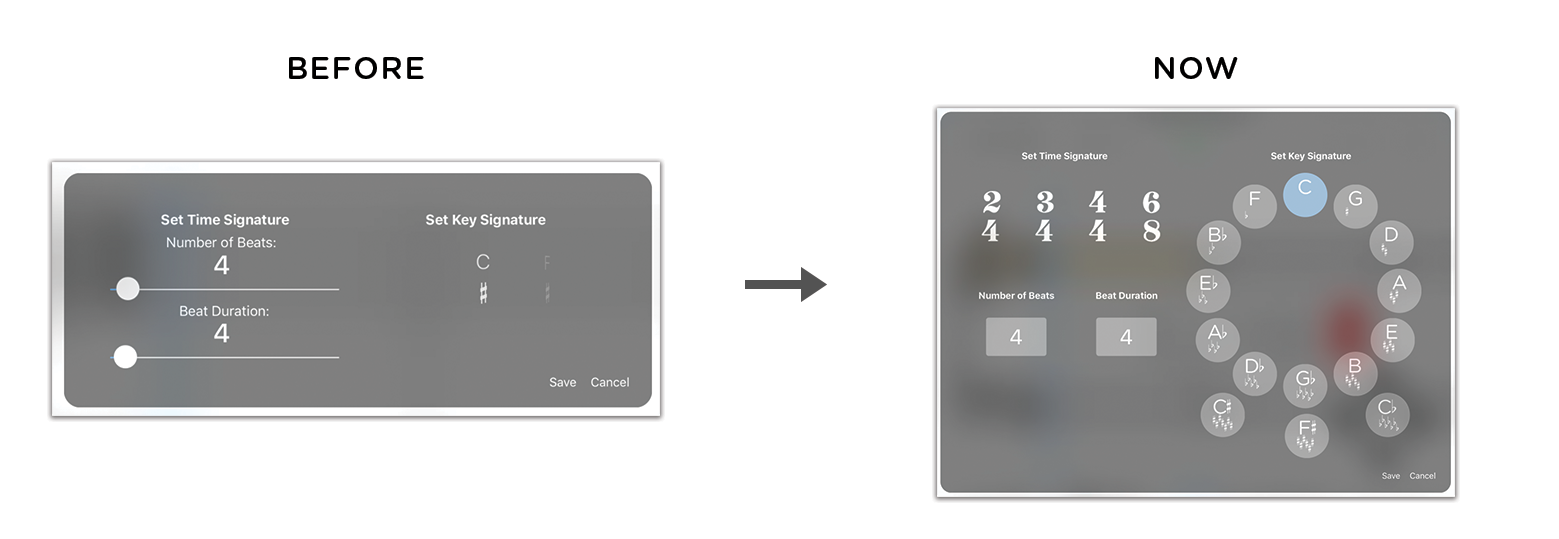
\includegraphics[scale=0.25]{figures/before-after-timesigmenu}
			    \caption{The time and key signature menu before and after changes were made due to the user testing. The revised time signature menu adds buttons for the common time signatures and also allows users to input any valid time signature they want. The revised key signature menu is now radial and follows the circle of fifths.}
			    \label{fig:time-key-signature}
			\end{figure} 

			The transposition interaction also needed improvement. In the iteration 1 and 2 prototype, users can tap on the up or down arrow keys to instantly transpose the selected notes to a higher or lower pitch respectively. It was observed that this was sometimes confusing and not easy to find. The confusion happened mainly because the users' assumption was that the arrow key was only used to move the cursor and not the notes. They would eventually be able to figure out after some messing around, but this still needed to be improved. Hence, in the succeeding iteration a menu was added containing the transpose arrow keys and other modifiers that would only appear when a user highlights a set of notes (see Figure \ref{fig:transpose}. This not only made it more obvious, but also saved space by only showing the necessary buttons when needed.

			\begin{figure}[h]
				\centering
				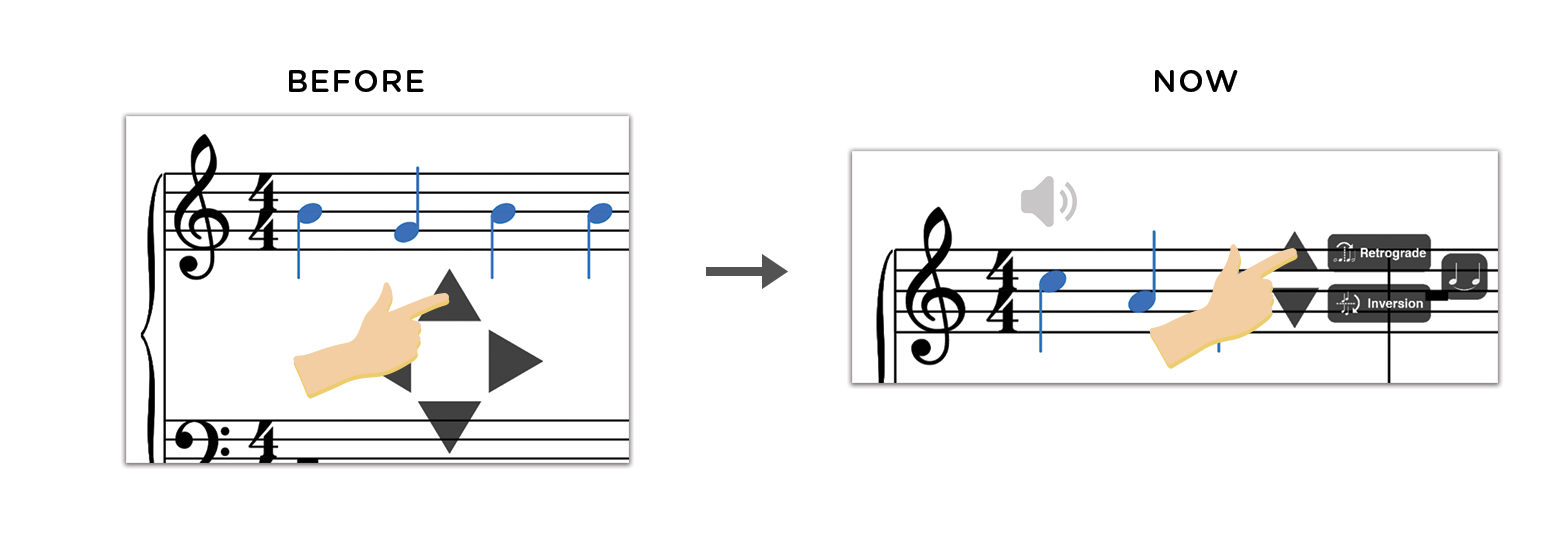
\includegraphics[scale=0.25]{figures/before-after-transpose-notes}
			    \caption{The transpose interaction before and after changes were made due to the user testing. The new transpose interaction adds a menu containing separate transpose arrow keys as well as additional modifiers.}
			    \label{fig:transpose}
			\end{figure}

			The feature that received the lowest score for this iteration was F19 (Remove an Accidental on a Highlighted/Selected Group of Notes). A lot of the composers said they felt that the buttons were too small and hard to press. However, the main problem with the feature was that the buttons were set up to follow music theory. In music theory, when a sharp is added to a note, it needs to be naturalized to remove the sharp. This was also the logic behind the accidentals in the prototype. When a note has a sharp, the user would have to press the naturalize button to remove it. Unfortunately, this was not obvious to the amateur users. They expected it to be similar to making a text bold or italicized in word processors. What they commonly did was when a note had a sharp, they would press the sharp button again to remove it. Since the buttons were not set up to follow it, nothing would happen and they thought that the buttons did not work. Expert composers, however, did not have a problem using this feature. When asked why they were able to figure it out easily, they mentioned that they just followed music theory. To suit both types of users, the prototype in the succeeding iterations also allowed users to press the accidental button again to remove an already placed accidental aside from the original method of removing accidentals.

			\begin{table}[!htpb]
			  \centering
			  \captionof{table}{Feature Related Questions for Iteration 2 Special Features} \label{tab:clerical-features}
			  \begin{tabular}{|R{1.5cm}|R{1cm}|R{1cm}|R{1cm}|R{1.5cm}|} \hline
			  	& \textbf{Q2} & \textbf{Q4} & \textbf{Q5} & \textbf{AveF} \\ \hline
			  	\textbf{F21} & 3.8 	& 3.8 	& 3.8 	& 3.80 \\ \hline
			    \textbf{F22} & 4.0 	& 4.0 	& 4.0 	& \textbf{4.00} \\ \hline
			    \textbf{F23} & 3.8 	& 3.8 	& 3.8 	& 3.80 \\ \hline
			    \textbf{F24} & 4.0 	& 4.0 	& 3.8 	& 3.93 \\ \hline
			    \textbf{F25} & 4.0 	& 4.0 	& 3.8 	& 3.93 \\ \hline
			    \textbf{F26} & 4.0 	& 4.0 	& 4.0 	& \textbf{4.00} \\  \hline
			    \textbf{F27} & 3.4 	& 3.4 	& 3.4 	& \textbf{3.40} \\ \hline
			    \textbf{AveQ} & 3.86 & 3.86 & 3.80 & \\ \hline
			  \end{tabular}
			\end{table}

			For features F21-F27, only Q2, Q4, and Q5 were used due to their nature of not being connected to the tasks and actual composition. Results for these features can be seen in Table \ref{tab:clerical-features}. Despite these features being new, they were simple enough to perform, hence the high scores.